\section{DS10}
\subsubsection{Blattgröße}
Blattgröße ist nicht Teil des „leaf economic spectrum“\\

\textbf{Palatabilität}\\
\textcolor{red}{Was ist Palatabilität?}
Palatabilität im Jahreslauf: Hohe Palatabilität (= hohe Sensitivität)\\
Mechanismus: Während der Differenzierung Aufbau der Sekundärwand und Einlagerung von Lignin\\
Hypothese: Bei größeren Blättern ist die sensitive Phase länger!\\

\textbf{Blattgröße \& Herbivorie}
\begin{itemize}
	\item \textbf{Große Blätter brauchen länger zur Entfaltung} (aber Steigung $<$ 1, d.h. pro Fläche ist die Enfaltungszeit bei großen Blättern kürzer)
	\item \textbf{Blätter längerer Entfaltungszeit mit höherem Blattverlust} (aber hohe Variabilität, weil Palatabilität auch von anderen Dingen abhängt)
\end{itemize}

\textbf{Anteil von Stütz(\& Leitungs-)gewebe:} Mit zunehmender Blattmasse ($\approx$ Blattfläche) nimmt der Masseanteil von Petiolus und Mittelrippe zu

\newpage
\textbf{Der „H tradoff“}
Ein hoher Stamm bedeutet:
\begin{itemize}
	\item Mehr Licht (+)
	\item Langsameres Wachstum wegen (–)
	\begin{itemize}
		\item Investition in Stamm
		\item Schutz des Kernholzes
		\item Zunehmend stärkerer Wasserspannung
	\end{itemize}
	\item Hohes Kavitationsrisiko (–)
	\item Hohes statisches Risiko (–)
\end{itemize}

\textbf{Holzdichte als „Mastervariable“}
\begin{itemize}
	\item „Positiv“:
	\begin{itemize}
		\item Statik (s.o.): Rigidität (versus Eigengewicht)
		\item Mechanische Belastbarkeit (z. B. Tritt, Schneebruch, Wind)
		\item Haltbarkeit gegen Zersetzung
		\item Zellstabilisierung bei Kavitation?
	\end{itemize}
	\item „Negativ“:
	\begin{itemize}
		\item Kostenfaktor C-Allokation
		\item Weniger „Platz“ für Leitgefäße, geringere Leitfähigkeit?
	\end{itemize}
\end{itemize}

\textbf{Holzdichte variiert regional}
\begin{itemize}
	\item variiert stärker als die Bestandesstruktur
	\item Biomasseunterschiede gehen auf Dichtemuster zurück (Leguminosen)
\end{itemize}

\textbf{Wachstum \& Mortalität = f(Holzdichte):} Bäume mit dichterem Holz wachsen langsamer, aber leben dafür länger\\
\textbf{Leitfähigkeit = f(Holzdichte):} Leitfähigkeit des Splintholzes $k_S$ sinkt mit der Holzdichte
\\\\
\underline{\textbf{Wichtige Ergebnisse}}
\begin{itemize}
	\item Positiver Zusammenhang zwischen Leitfähigkeit und Wachstum (erstmals gezeigt)
	\item Nichts Neues: Dichte hat negativen Zusammenhang (evt. über Leitfähigkeit) zu Wachstum und positiven zu Überlebensrate
	\item Überleben hat nichts mit dem Parenchymanteil zu tun („Speicher“)
\end{itemize}

\subsubsection{Biodiversität und Klima}
\begin{itemize}
	\item Erstes BDEF-Thema: Vegetationseffekte auf das Klima
	\item Wie Diversität ins Spiel kommt...
	\item Beispiele
	\item Diversität in Modellen
\end{itemize}

\textbf{Die Hauptpfade}
\begin{itemize}
	\item Energiebilanz
	\item Kohlenstoff-Klima Interaktion
\end{itemize}

\textbf{Energiebilanz}\\
\begin{figure}[htp]
\centering
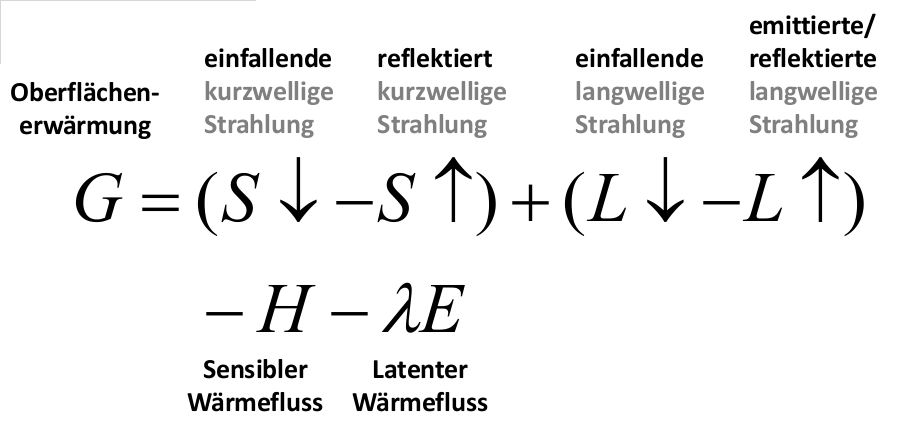
\includegraphics[scale=0.5]{lectures/DS10/pix/energybalance.png}
\caption{}
\label{}
\end{figure}

\textcolor{blue}{\textbf{Zusammenfassung siehe Vorlesung}}
\\\\
\textcolor{red}{Was kann man aus der Vorlesung sonst noch so mitnehmen???}
\\\\
\textbf{Die wirkliche Herausforderung} Gibt es Klimaunterschiede durch regionale Diversitäts-/Identitätsunterschiede?